\section{Evaluation}
\label{sec:Evaluation}

Ziel dieses Kapitels ist die systematische Bewertung des entwickelten Chatbots zur Unterstützung bei vergaberechtlichen Fragestellungen. Die Evaluation erfolgt auf zwei Ebenen: der Qualität der Dokumentenretrieval-Komponente sowie der Qualität der generierten Antworten. Hierfür werden sowohl klassische Information-Retrieval-Metriken als auch ein LLM-as-a-Judge-Ansatz eingesetzt.

\subsection{Evaluationsmethodik}

Die Evaluation basiert auf einem Datensatz realistischer Nutzeranfragen einschließlich der zugehörigen Referenzantworten sowie relevanter Ground-Truth-Dokumente. Ziel ist es, die Leistungsfähigkeit des entwickelten Retrieval-Augmented-Generation-(RAG)-Systems sowohl hinsichtlich der Dokumentensuche als auch der Antwortgenerierung systematisch zu bewerten.

Der Evaluationsaufbau orientiert sich an einem strukturierten Benchmark-Ansatz, um reproduzierbare und vergleichbare Ergebnisse zu gewährleisten. Hierzu werden die Anfragen in zwei Kategorien unterteilt: domänenspezifische, kontextbezogene Fragen aus dem Bereich des Vergaberechts sowie domänenfremde, kontextunabhängige Fragen. Diese Trennung ermöglicht eine differenzierte Analyse der fachlichen Antwortqualität sowie der Robustheit des Systems gegenüber irrelevanten oder außerhalb der Wissensbasis liegenden Eingaben.

Für jede Anfrage werden im Rahmen der Evaluation die folgenden Komponenten systematisch erfasst und gespeichert:
\begin{itemize}
    \item die ursprüngliche Nutzeranfrage,
    \item die durch das Retrieval-Modul identifizierten Dokumente,
    \item die generierte Antwort des Sprachmodells,
    \item sowie Referenzantworten bzw.\ relevante Ground-Truth-Dokumente.
\end{itemize}

Die Verarbeitung und Speicherung der Ergebnisse erfolgt in strukturierten JSON-Dateien. Dies ermöglicht eine automatisierte Auswertung sowie eine vollständige Nachvollziehbarkeit und Reproduzierbarkeit der Experimente.

Zur Bewertung des Systems kommen zwei komplementäre Ansätze zum Einsatz. Einerseits wird die Qualität des Retrievals mithilfe klassischer Information-Retrieval-Metriken wie Precision@k und Recall@k gemessen. Andererseits wird die Qualität der generierten Antworten durch einen LLM-as-a-Judge-Ansatz bewertet.

Die Antwortgenerierung erfolgt durch das Sprachmodell \textit{gpt-oss} (20B). Die Bewertung der generierten Antworten wird durch ein separates Sprachmodell (\textit{llama3.1:8b}) durchgeführt. Durch diese Trennung von Generierung und Bewertung wird eine methodisch fundierte und vergleichsweise objektive Einschätzung der Antwortqualität ermöglicht.

Der Datensatz umfasst unter anderem folgende Anfragen:

\textbf{Fragen im Kontext:}
\begin{enumerate}
    \item Ab welchem Betrag ist eine Vergabe durchzuführen (UVgO, VVÖA, LHO)?
    \item Ab welchem Betrag ist eine Beschaffung durchzuführen (UVgO, VVÖA, LHO)?
    \item Wie lange dauert ein Vergabeverfahren (UVgO, VgV)?
    \item Ist der Höchstbetrag in Brutto oder Netto anzugeben (UVgO, VgV, VVÖA)?
    \item Warum ist ein Vergabeverfahren durchzuführen (LHO, UVgO, VgV, VVÖA)?
    \item Welcher Preis ist zu beachten (VV~ÖA)?
    \item Als Mitarbeitender oder Professorin möchte ich wissen, ob Beträge, Preise und Kostenschätzungen in Brutto oder Netto anzugeben sind, um das korrekte Verfahren bestimmen zu können.
    \item Als Institutssekretariat möchte ich wissen, welche Dokumente der Beschaffungsstelle vorgelegt werden müssen, um eine Bestellung rechtssicher einzuleiten.
    \item Als wissenschaftlich Mitarbeitender möchte ich wissen, wie lange eine Ausschreibung offen sein muss und welche Fristen für Angebotsabgabe und Zuschlag gelten.
    \item Als wissenschaftlich Mitarbeitende möchte ich erfahren, ob Angebote selbst eingeholt werden dürfen oder ob dies durch die Beschaffungsstelle erfolgt.
    \item Als Projektleiterin oder Mitarbeitender möchte ich verstehen, was ein Vergabeverfahren bzw.\ eine Beschaffung im Kontext der Vergaberegelungen bedeutet.
    \item Als Projektleiter*in einer rheinland-pfälzischen Hochschule möchte ich wissen, warum Vergabeverfahren durchgeführt werden müssen und warum eine direkte Vergabe an einen Wunschlieferanten nicht zulässig ist.
\end{enumerate}

\textbf{Fragen außerhalb des Kontexts:}
\begin{enumerate}
    \item Wie mache ich eine Mondlandung?
    \item Wie koche ich Pasta?
    \item Wer hat die Relativitätstheorie erfunden?
    \item Wie repariere ich einen kaputten Laptop?
    \item d
\end{enumerate}

Durch die Kombination aus Retrieval-Evaluation und LLM-basierter Antwortbewertung wird ein ganzheitliches Benchmarking des Systems entlang der gesamten RAG-Pipeline ermöglicht. Dies erlaubt sowohl die isolierte Analyse einzelner Komponenten als auch die Untersuchung ihrer Wechselwirkungen innerhalb der Gesamtarchitektur.

\subsection{Bewertungsmetriken}

Zur Bewertung wurden zwei zentrale Ansätze verwendet:

\textbf{Klassische Information-Retrieval-Metriken (Precision@k, Recall@k)}\
Diese Metriken messen die Qualität der Dokumentensuche. Precision@k gibt an, wie viele der Top- k  zurückgegebenen Dokumente relevant sind, während Recall@k den Anteil der insgesamt relevanten Dokumente misst, der in den Top- k  enthalten ist. Die Relevanz wurde zweistufig definiert:
\begin{itemize}
    \item \textit{Mode A (streng)}: Nur Dokumente mit \texttt{relevanz=hoch} gelten als relevant.
    \item \textit{Mode B (moderat)}: Dokumente mit \texttt{relevanz=hoch} oder \texttt{relevanz=mittel} gelten als relevant.
\end{itemize}

\textbf{LLM-basierte Bewertung der Antwortqualität (LLM-as-a-Judge)}\
Für die Bewertung der Antwortqualität wurde ein lokal ausgeführtes LLM (\texttt{llama3.1:8b}) verwendet. Das Modell fungiert als unabhängiger Gutachter und bewertet die generierten Antworten auf Basis eines strukturierten Prompts anhand von vier Kriterien auf einer Skala von 1 (schlecht) bis 5 (sehr gut):

\begin{description}
    \item[Correctness (Korrektheit):] Ist die Antwort fachlich korrekt basierend auf den Quellen?
    \item[Completeness (Vollständigkeit):] Beantwortet die Antwort die Frage vollständig?
    \item[Faithfulness (Faktentreue):] Bleibt die Antwort treu zu den gegebenen Quellen (keine Halluzinationen)?
    \item[Clarity (Klarheit):] Ist die Antwort klar, strukturiert und verständlich?
\end{description}

Durch den Einsatz eines separaten Modells wird eine objektivere Einschätzung der Antwortqualität ermöglicht, da die Bewertung unabhängig vom generierenden System erfolgt.

Die Ergebnisse wurden in JSON-Dateien gespeichert und anschließend automatisiert ausgewertet. Die Auswertung erfolgt getrennt für Kontextfragen und Out-of-Context-Fragen, um ein differenziertes Bild der Systemleistung zu erhalten.

\subsection{Retrieval-Evaluation}

Zur Bewertung der Suchqualität werden die Metriken Precision@k und Recall@k herangezogen. Diese quantifizieren den Anteil relevanter Dokumente innerhalb der Top- k -Ergebnisse sowie die Abdeckung aller relevanten Dokumente.

\begin{itemize}
    \item Precision@k = relevante Treffer in Top- k  /  k 
    \item Recall@k = relevante Treffer in Top- k  / Gesamtanzahl relevanter Dokumente
\end{itemize}

Die dargestellten Ergebnisse basieren auf aggregierten Durchschnittswerten über mehrere evaluierte Anfragen. Für jeden  k -Wert wurden Precision und Recall über alle betrachteten Fragen gemittelt, um eine vergleichbare Bewertung der Retrieval-Leistung zu ermöglichen.

Die Ergebnisse für die In-Context-Fragen weisen auf eine sehr hohe Retrieval-Qualität hin. Über alle betrachteten  k -Werte hinweg erreicht das System eine konstante Precision von 1{,}0, was bedeutet, dass ausschließlich relevante Dokumente unter den Top- k -Ergebnissen enthalten sind.

Der Recall steigt mit zunehmendem  k  kontinuierlich an. Während bei  k=1  lediglich ein kleiner Teil der relevanten Dokumente identifiziert wird (Recall@1 = 0{,}07), erhöht sich die Abdeckung sukzessive. Bei  k=10  werden bereits rund zwei Drittel der relevanten Dokumente gefunden, und bei  k=15  wird schließlich ein vollständiger Recall von 1{,}0 erreicht. Dies deutet darauf hin, dass relevante Dokumente zuverlässig im Ranking enthalten sind, jedoch nicht immer auf den obersten Positionen erscheinen.

\begin{figure}[H]
\centering
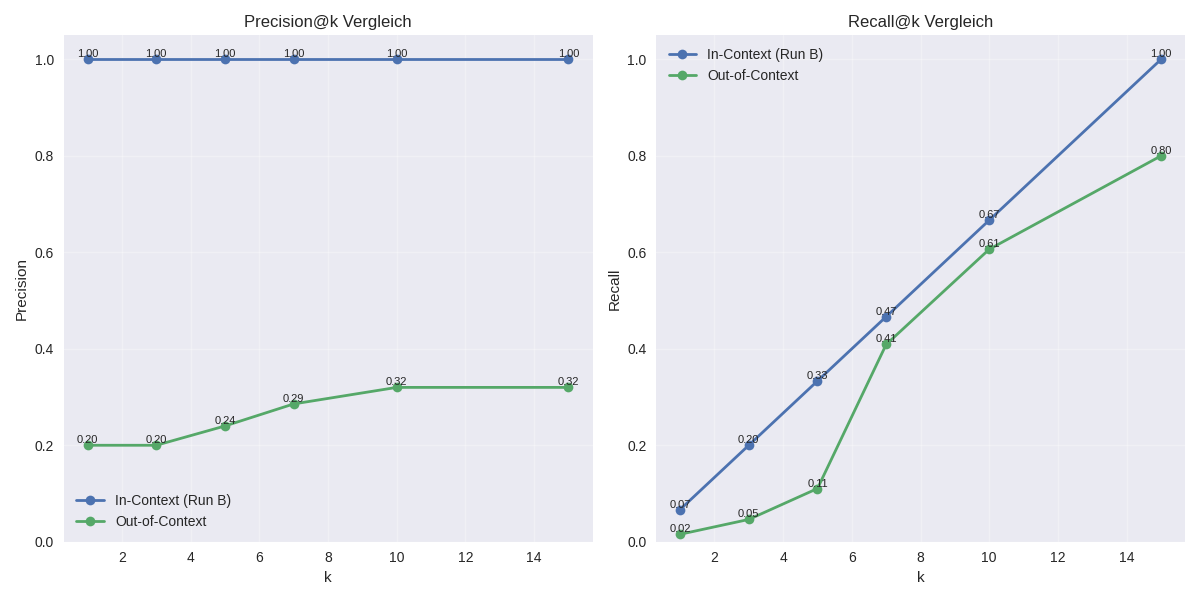
\includegraphics[width=0.9\textwidth]{precrecall.png}
\caption{Precision@k und Recall@k für verschiedene Werte von  k  (Vergleich von In-Context- und Out-of-Context-Fragen)}
\label{fig:precision_recall1}
\end{figure}

Im Gegensatz dazu weisen die Ergebnisse für die Out-of-Context-Fragen auf eine deutlich geringere Retrieval-Qualität hin. Die Precision liegt bei kleinen  k -Werten bei etwa 0{,}20 und steigt nur moderat auf rund 0{,}32 bei größeren  k -Werten. Dies verdeutlicht, dass ein erheblicher Anteil der zurückgegebenen Dokumente nicht relevant ist.

Auch der Recall ist für Out-of-Context-Anfragen zunächst sehr gering (Recall@1 = 0{,}02), steigt jedoch mit wachsendem  k  deutlich an und erreicht bei  k=15  einen Wert von etwa 0{,}80. Dieser Anstieg ist jedoch mit einer vergleichsweise niedrigen Precision verbunden, was darauf hinweist, dass relevante Dokumente erst durch eine größere Anzahl zusätzlicher, teilweise irrelevanter Treffer gefunden werden.

Insgesamt weisen die Ergebnisse darauf hin, dass die Retrieval-Leistung vom Kontext der Anfrage beeinflusst wird. Während In-Context-Fragen mit hoher Präzision und wachsendem Recall beantwortet werden können, führt das Fehlen eines passenden Kontexts bei Out-of-Context-Anfragen zu einer geringeren Ergebnisqualität.

\clearpage
\subsubsection{Analyse der Hybrid-Suche}

Die Analyse des Überlappungsgrades zwischen BM25 und Vektorsuche zeigt insgesamt eine geringe Überschneidung der identifizierten Dokumente und verdeutlicht die unterschiedlichen Eigenschaften beider Retrieval-Ansätze.

Für die In-Context-Anfrage zeigt sich eine teilweise Überschneidung der Ergebnisse. Wie in Abbildung~\ref{fig:bm25_vector_in} dargestellt, werden drei Dokumente von beiden Verfahren identifiziert, was einem Überlappungsgrad von etwa 23,% entspricht. Gleichzeitig existieren mehrere Dokumente, die ausschließlich von einem der beiden Verfahren gefunden werden.

Dies verdeutlicht die komplementären Eigenschaften der Ansätze: Während BM25 auf exakten Termübereinstimmungen basiert, erfasst die Vektorsuche semantische Zusammenhänge. Die Kombination beider Verfahren ermöglicht somit eine breitere Abdeckung relevanter Dokumente.

\begin{figure}[H]
    \centering
    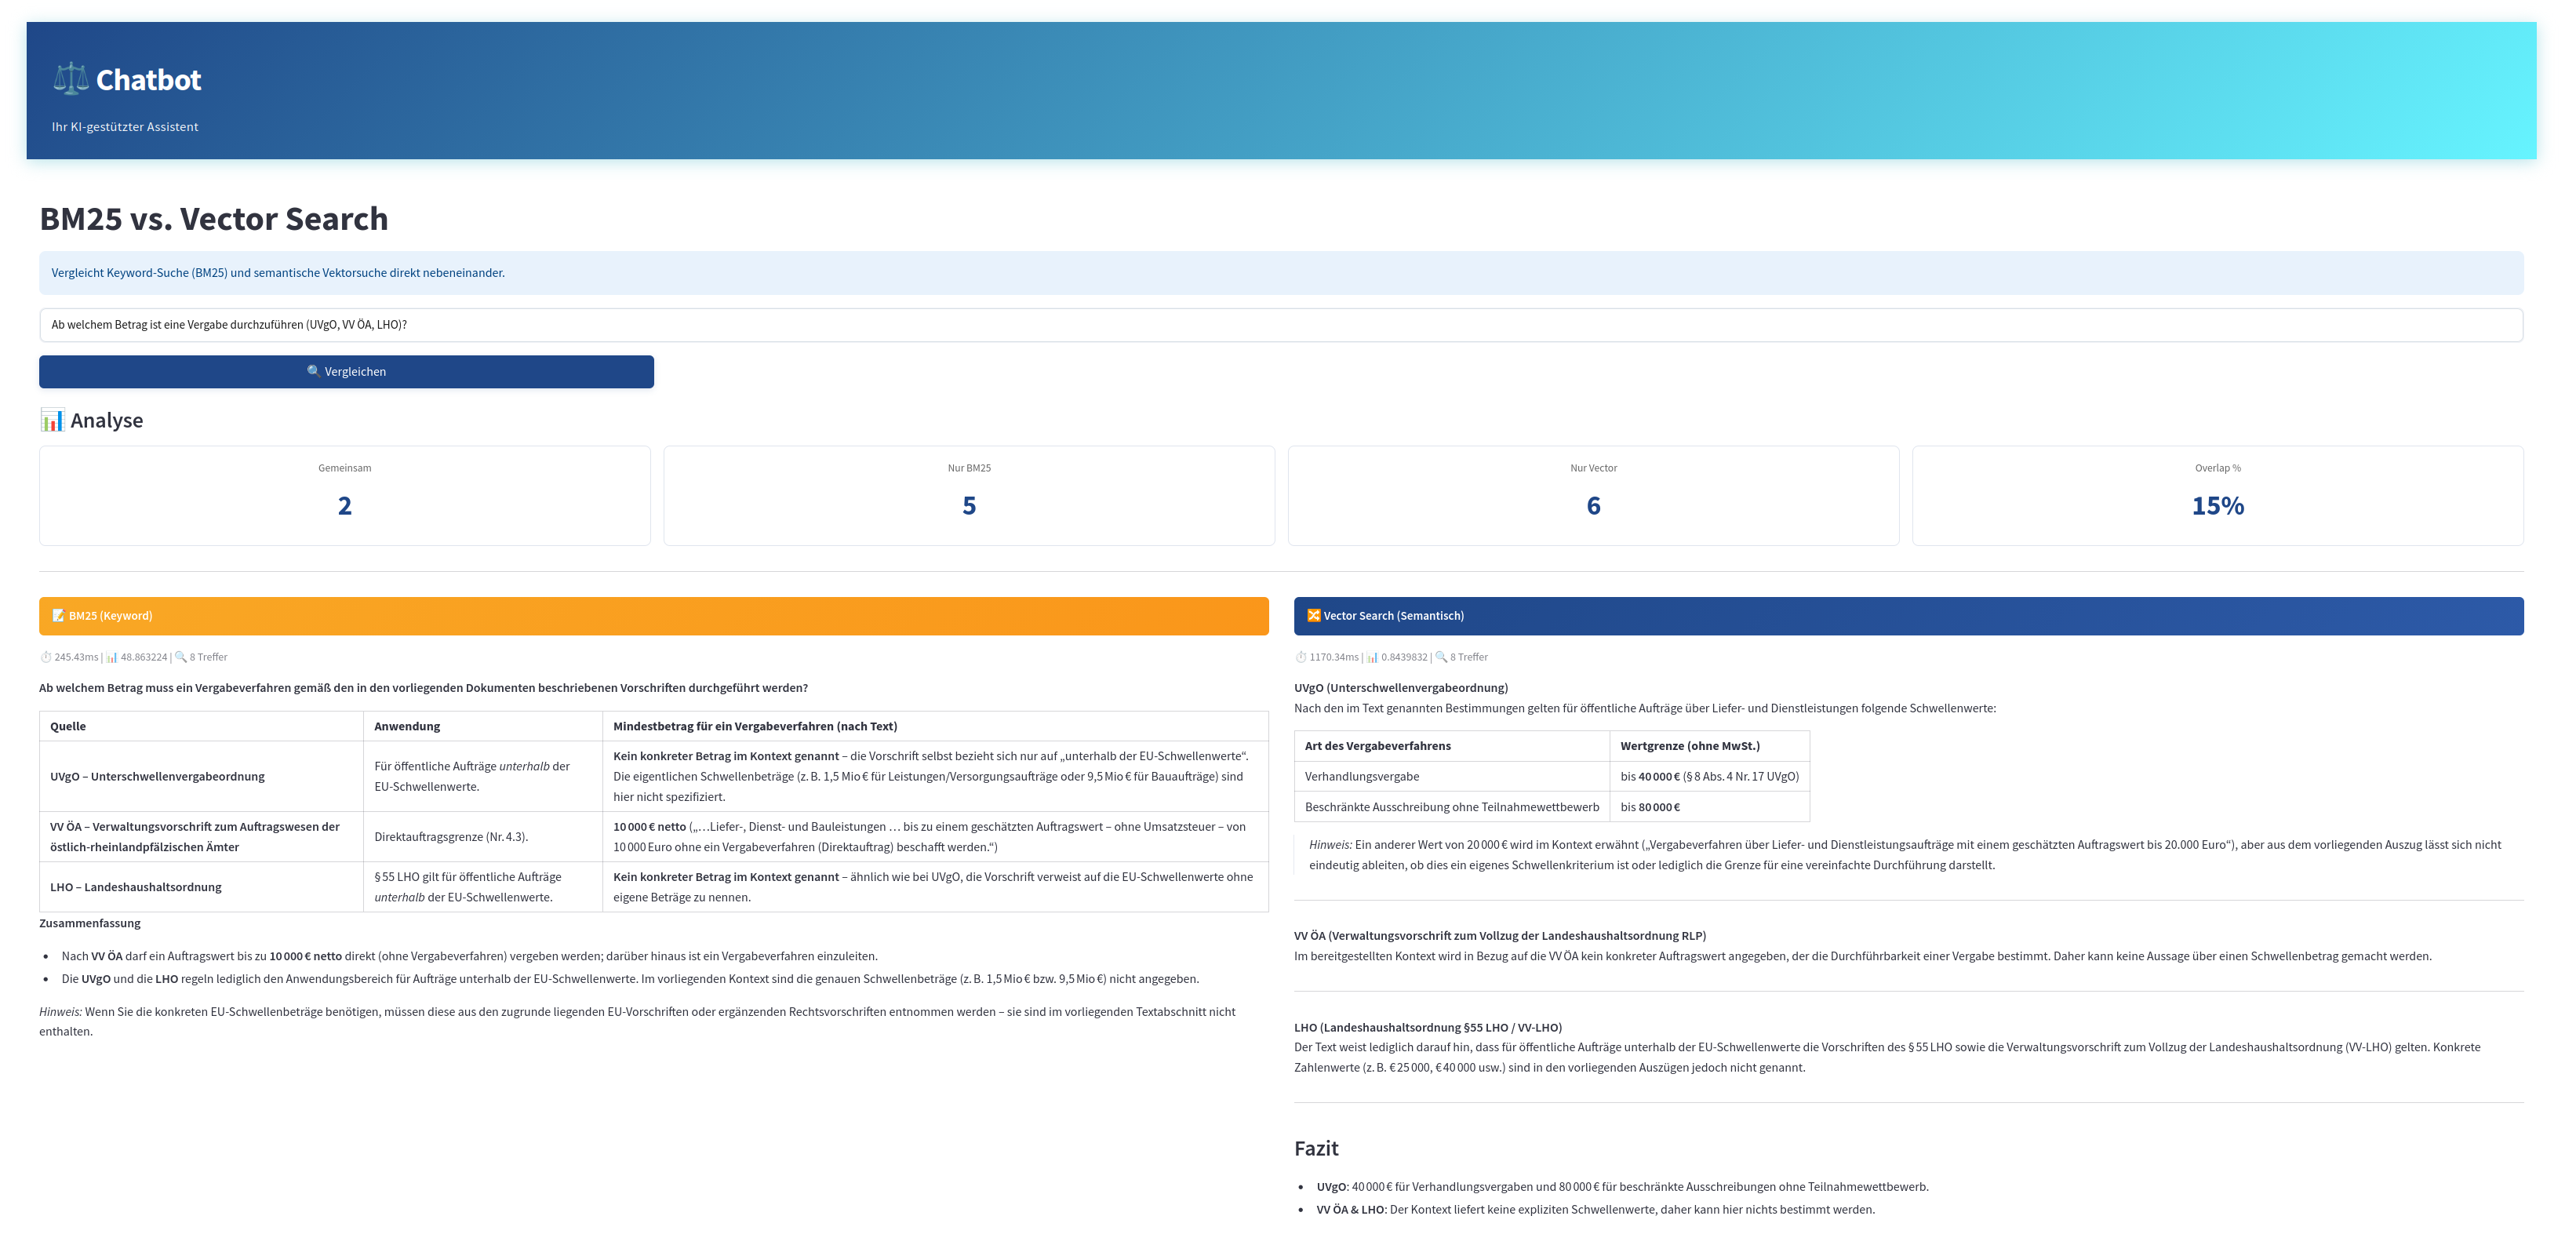
\includegraphics[width=0.9\textwidth]{Vergleich_BM25_Vector.png}
    \caption{Vergleich der Retrieval-Ergebnisse von BM25 und Vektorsuche für eine In-Context-Anfrage ( k=5 )}
    \label{fig:bm25_vector_in}
\end{figure}

Im Gegensatz dazu zeigt die Out-of-Context-Anfrage eine vollständige Divergenz der Ergebnisse. Wie in Abbildung~\ref{fig:bm25_vector_out} zu sehen ist, existiert keine Überschneidung zwischen den von BM25 und der Vektorsuche identifizierten Dokumenten (0,\%).

Dieses Verhalten unterstreicht die unterschiedlichen Suchprinzipien besonders deutlich: Ohne passenden Kontext greifen die Verfahren auf verschiedene, jeweils nicht optimal geeignete Relevanzsignale zurück.

\begin{figure}[H]
    \centering
    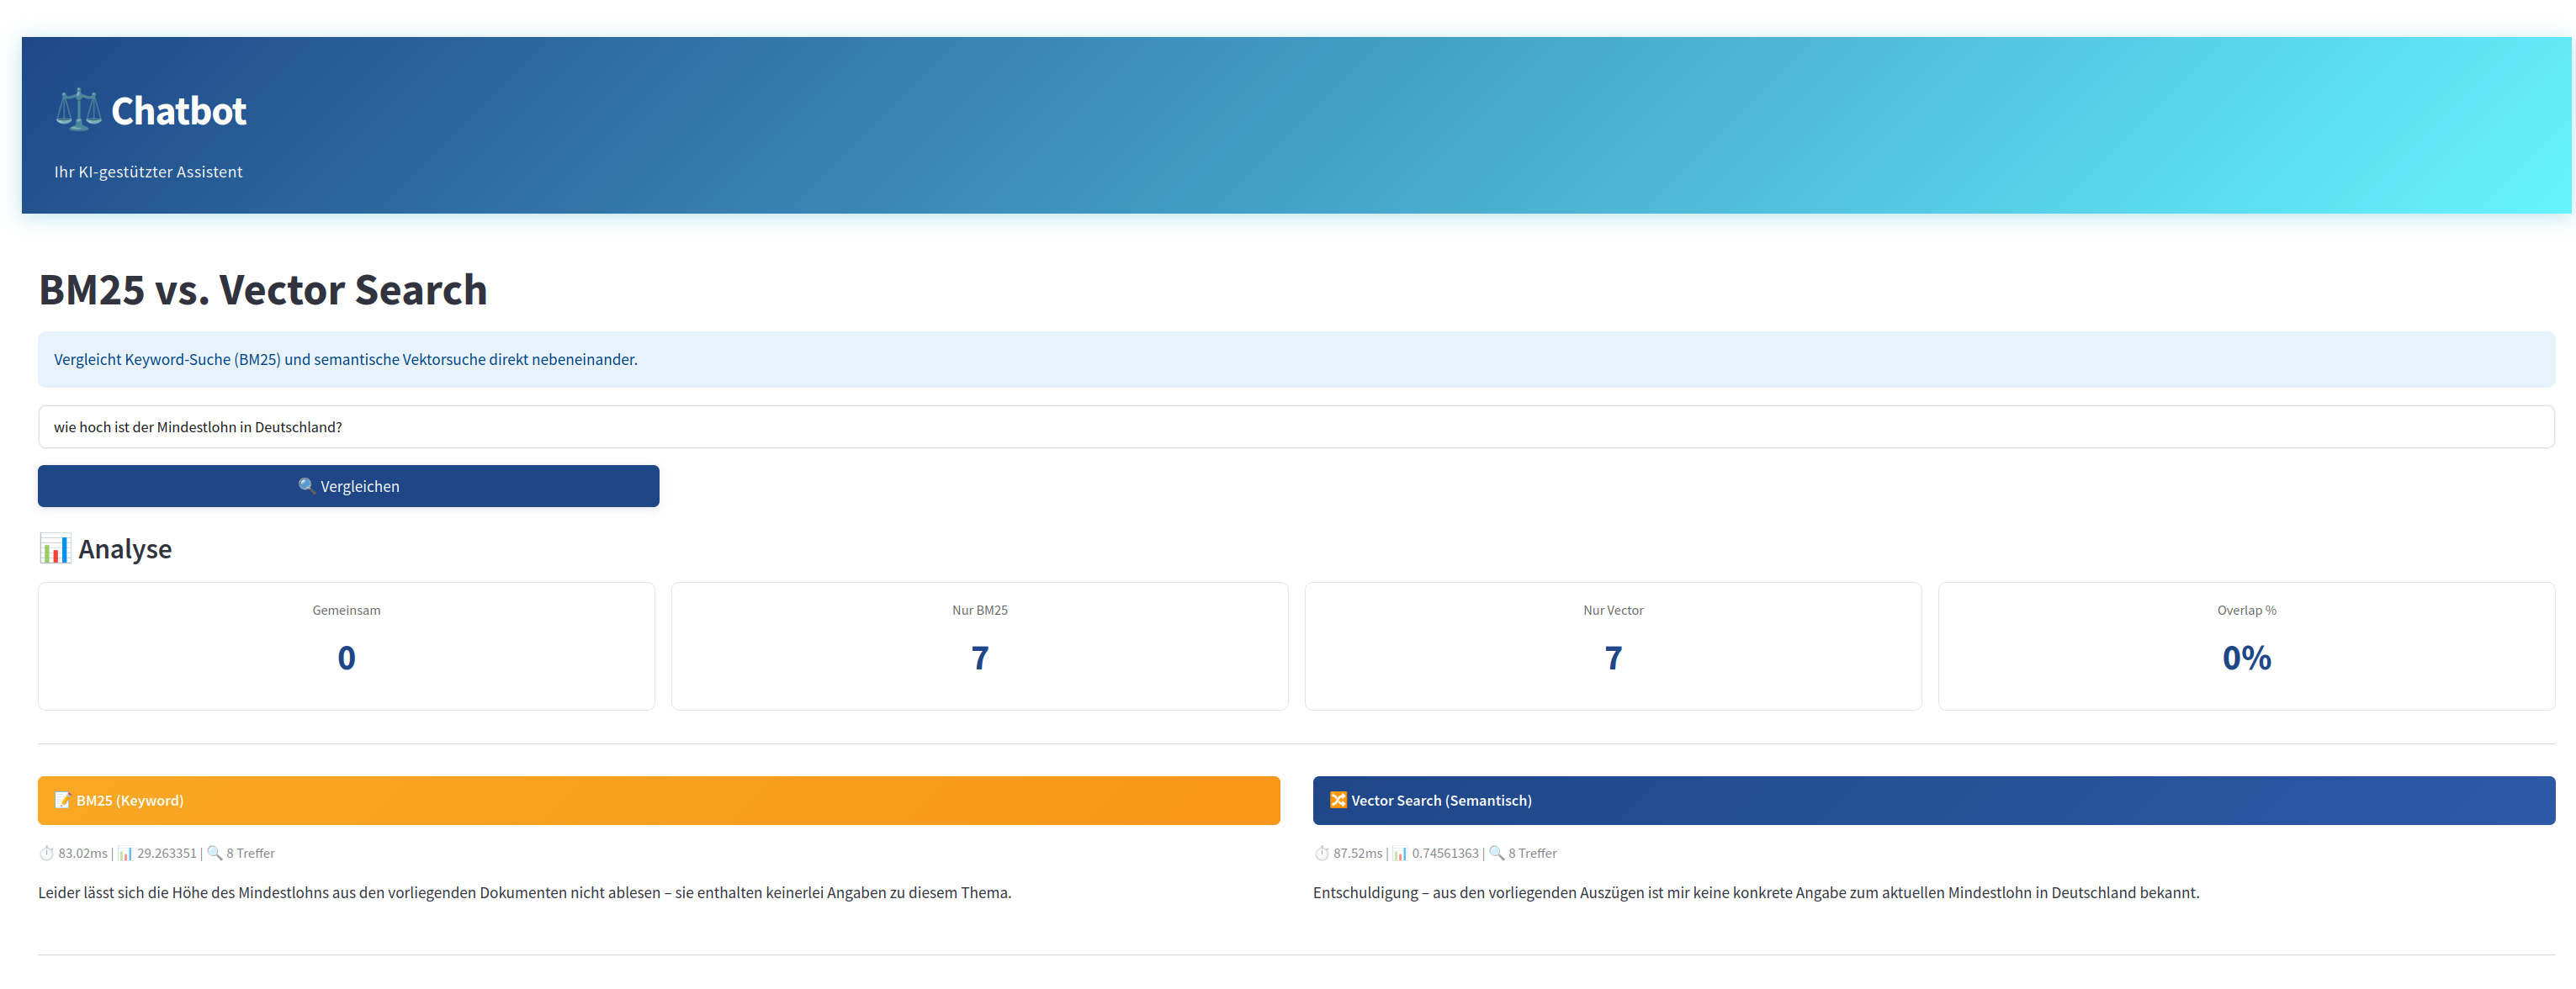
\includegraphics[width=0.9\textwidth]{out_bm25_vector.png}
    \caption{Vergleich der Retrieval-Ergebnisse von BM25 und Vektorsuche für eine Out-of-Context-Anfrage ( k=5 )}
    \label{fig:bm25_vector_out}
\end{figure}

Insgesamt legen die Ergebnisse nahe, dass BM25 und Vektorsuche komplementäre Eigenschaften aufweisen und ihre Kombination zu einer verbesserten Abdeckung relevanter Dokumente beitragen kann.

\subsection{Ergebnisse der Antwortbewertung}

Zur Bewertung der generierten Antworten wird ein LLM-as-a-Judge-Ansatz eingesetzt. Die Antworten werden durch das Modell \textit{gpt-oss} (20B) generiert und anschließend durch \textit{llama3.1:latest} bewertet.

Die Bewertung erfolgt anhand der folgenden Kriterien:

\begin{itemize}
    \item Correctness (fachliche Korrektheit)
    \item Completeness (inhaltliche Vollständigkeit)
    \item Faithfulness (Quellentreue)
    \item Clarity (Verständlichkeit und Struktur)
\end{itemize}

Die dargestellten Ergebnisse basieren auf aggregierten Durchschnittswerten über mehrere evaluierte Fragen. Für jede Kategorie wurde der arithmetische Mittelwert der durch das LLM vergebenen Bewertungen berechnet, um eine vergleichbare Gesamtbewertung der Antwortqualität zu ermöglichen.

Die Ergebnisse werden getrennt für In-Context- und Out-of-Context-Fragen betrachtet.

Für die In-Context-Fragen zeigt sich ein insgesamt hohes Qualitätsniveau:

\begin{itemize}
    \item Correctness: 4{,}75
    \item Completeness: 4{,}33
    \item Faithfulness: 4{,}33
    \item Clarity: 4{,}67
\end{itemize}

Dies entspricht einer Gesamtbewertung von 4{,}52 von 5{,}0 Punkten (vgl. Abbildung~\ref{fig:judge_scores_in}).

\begin{figure}[h]
    \centering
    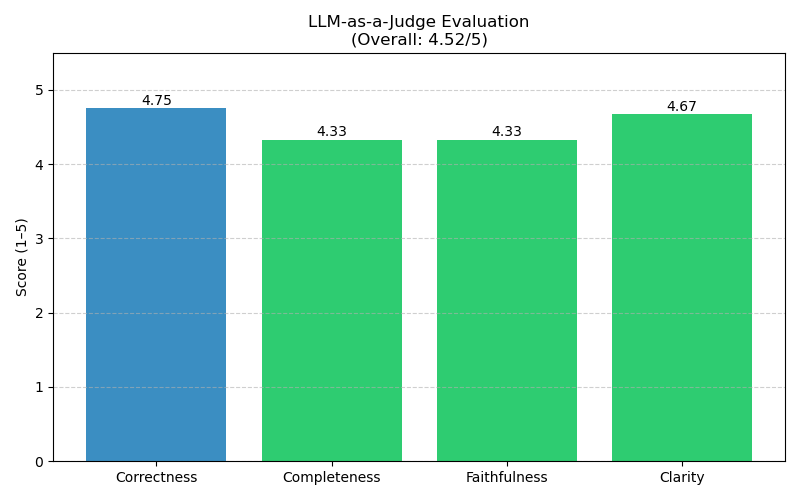
\includegraphics[width=0.75\textwidth]{judge_scores_in_context.png}
    \caption{LLM-basierte Bewertung der Antwortqualität für In-Context-Fragen}
    \label{fig:judge_scores_in}
\end{figure}

Die Ergebnisse zeigen, dass die generierten Antworten überwiegend fachlich korrekt, klar strukturiert und eng an den zugrunde liegenden Quellen orientiert sind. Leichte Abweichungen zeigen sich insbesondere bei der Vollständigkeit und Quellentreue.

Für Out-of-Context-Fragen ergibt sich hingegen ein deutlich geringerer Gesamtscore:

\begin{itemize}
    \item Correctness: 2{,}80
    \item Completeness: 2{,}60
    \item Faithfulness: 5{,}00
    \item Clarity: 4{,}40
\end{itemize}

Dies entspricht einer Gesamtbewertung von 3{,}70 von 5{,}0 Punkten (vgl. Abbildung~\ref{fig:judge_scores_out}).

\begin{figure}[h]
    \centering
    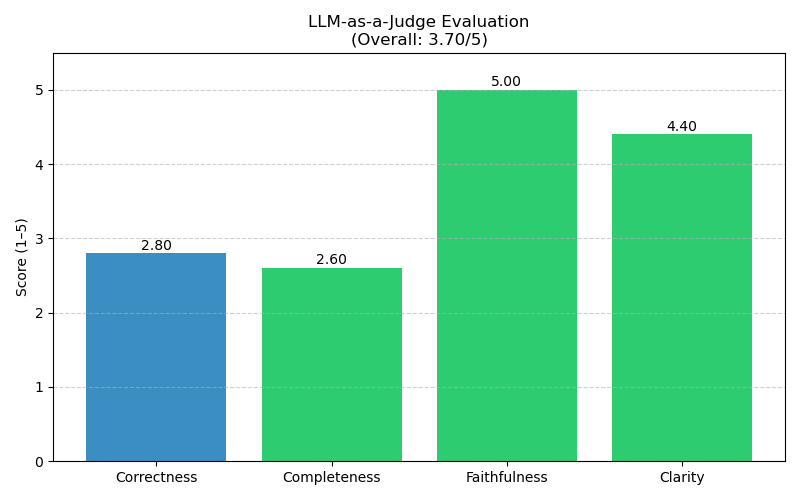
\includegraphics[width=0.75\textwidth]{judge_scores_out_context.png}
    \caption{LLM-basierte Bewertung der Antwortqualität für Out-of-Context-Fragen}
    \label{fig:judge_scores_out}
\end{figure}

Auffällig ist insbesondere die konstant hohe Bewertung der Faithfulness bei Out-of-Context-Fragen. Dies deutet darauf hin, dass das System keine nicht durch den Kontext gestützten Informationen generiert und somit ein robustes Verhalten gegenüber Halluzinationen aufweist.

Es ist jedoch zu beachten, dass durch die Verwendung von Durchschnittswerten individuelle Abweichungen einzelner Antworten nicht im Detail sichtbar werden. Die Ergebnisse liefern daher primär eine aggregierte Einschätzung der Systemleistung.

Insgesamt verdeutlichen die Ergebnisse, dass die Qualität der generierten Antworten maßgeblich von der Verfügbarkeit relevanter Kontextinformationen abhängt.

\subsubsection{Qualitative Analyse}

Die qualitative Analyse zeigt zwei zentrale Verhaltensweisen des Systems.

Zum einen erkennt das System Situationen, in denen die bereitgestellten Kontextinformationen nicht ausreichen, und kommuniziert diese Unsicherheit explizit. Dieses Verhalten trägt zur Reduktion von Halluzinationen bei.

Zum anderen werden in Einzelfällen zusätzliche Informationen generiert, die nicht vollständig durch die zugrunde liegenden Quellen abgesichert sind. Dies verdeutlicht die inhärenten Grenzen des Systems im Umgang mit unvollständigem Kontext.

\subsection{Diskussion}

Die Kombination aus Retrieval-Metriken und LLM-basierter Bewertung ermöglicht eine differenzierte Analyse der Systemleistung.

Während Precision@k und Recall@k die Effektivität der Dokumentensuche quantifizieren, bewertet der LLM-as-a-Judge-Ansatz die Nutzbarkeit der generierten Antworten auf Basis aggregierter Durchschnittswerte.

Die Ergebnisse deuten darauf hin, dass die hybride Suche zur Verbesserung der Retrieval-Abdeckung beiträgt, indem unterschiedliche Stärken von BM25 und Vektorsuche kombiniert werden.

Zudem zeigt sich ein Zusammenhang zwischen der Qualität der Retrieval-Ergebnisse und der Qualität der generierten Antworten. Insbesondere bei fehlendem oder unzureichendem Kontext sinkt die Antwortqualität.

Die beobachteten Einschränkungen in der Vollständigkeit können im Kontext der verwendeten RAG-Architektur interpretiert werden und stehen im Zusammenhang mit der Verfügbarkeit relevanter Dokumente.

\subsection{Zusammenfassung}

Zusammenfassend lässt sich festhalten, dass das entwickelte System in den durchgeführten Evaluationsszenarien insgesamt gute Ergebnisse erzielt.

Die Hybrid-Suche ermöglicht die zuverlässige Identifikation relevanter Dokumente und erreicht bei höheren  k -Werten einen vollständigen Recall. Die generierten Antworten weisen insgesamt eine hohe fachliche Qualität sowie eine ausgeprägte Quellentreue auf.

Einschränkend ist anzumerken, dass der Evaluationsdatensatz mit drei Testfragen nur eine begrenzte Aussagekraft besitzt. Zudem können durch die Verwendung von Durchschnittswerten individuelle Abweichungen einzelner Bewertungen nicht vollständig abgebildet werden.

Eine Erweiterung des Datensatzes sowie die Einbeziehung menschlicher Evaluationen stellen sinnvolle Ansätze für zukünftige Arbeiten dar.

Insgesamt legen die Ergebnisse nahe, dass die Kombination aus Hybrid-Retrieval und LLM-basierter Antwortgenerierung eine geeignete Grundlage für ein domänenspezifisches Expertensystem im vergaberechtlichen Kontext darstellen kann.
\clearpage